\documentclass[a4paper, 12pt]{article}

\usepackage[table,xcdraw]{xcolor}
\usepackage[left=2.5cm, right=1.5cm, top=1.5cm, bottom=1.5cm]{geometry}
\usepackage{graphicx}
\usepackage{xcolor}
\usepackage{mdframed}
\usepackage { amsmath , amssymb , amsthm }
\usepackage[T2A]{fontenc}
\usepackage[utf8]{inputenc}
\usepackage[english,russian]{babel}
\usepackage{listings}
\usepackage{setspace}
\usepackage{amsmath}
\usepackage{float}
\usepackage{multirow}
\usepackage{lscape}


\onehalfspacing
\renewcommand{\familydefault}{\sfdefault}
% \renewcommand{\familydefault}{\sffamily}

\graphicspath{{img/}}
\DeclareGraphicsExtensions{.pdf,.png,.jpg}


\begin{document}
\begin{titlepage}
  \begin{center}
    \MakeUppercase{Министерство науки и высшего образования Российской Федерации} \\
    \MakeUppercase{ФГБОУ ВО Алтайский госудаственный университет}
    \vspace{0.25cm}
    
	  Институт цифровых технологий, электроники и физики
    
    Кафедра вычислительной техники и электроники
    \vfill
    
    {\LARGE Лабораторная работа №1. Графический метод решения задач линейного программирования}\\[5mm]
    \textsc{(Отчёт по лабораторным работам по курсу <<Методы оптимизации>>. \\13 вариант)}
  \bigskip

\end{center}
\vfill

\newlength{\ML}
\settowidth{\ML}{«\underline{\hspace{0.7cm}}» \underline{\hspace{1cm}}}
\hfill
\begin{minipage}{0.45\textwidth}
  Выполнил: ст. 595 гр.:\\
  \underline{\hspace{\ML}} Д.\,В.~Осипенко\\
  Проверил: к.ф-м. наук, доцент каф. ВТиЭ\\
  \underline{\hspace{\ML}} В.\,И.~Иордан\\
  «\underline{\hspace{0.7cm}}» \underline{\hspace{2cm}} \the\year~г.
\end{minipage}%
\vfill

\begin{center}
  Барнаул, \the\year~г.
\end{center}
\end{titlepage}

\newpage

\section{Краткие теоретические сведения по теме лабораторной работы}
Пусть необходимо найти максимальное значение функции $Z(x) =c_1x_1 + c_2x_2 $ при ограничениях:\\

\begin{math}
  \begin{cases}
    a_{11}x_1+a_{12}x_2 \leq b_1\\
    a_{21}x_1+a_{22}x_2 \leq b_2\\
    \ldots\\
    a_{m1}x_1+a_{m2}x_2 \leq b_m\\
  \end{cases}
  \quad
  x_1 \geq 0, x_2 \geq 0
\end{math}\\

Допустим, что система ограничений имеет решение, а ее многоугольник решений ограничен.

Каждое из неравенств ограничений определяет полуплоскость с границей $a_{i1}+x_1+a{i2}x_2 = b_i, i=1\ldots m$ или $x_1=0,x_2=0$

Так как множество точек пересечения данных полуплоскостей - выпуклое, то областью допустимых решений задачи является выпуклое множество, которое называется многоугольником решений. Стороны этого многоугольника лежат на прямых, уравнения которых получаются из исходной системы ограничений заменой знаков неравенств на знаки точных равенств.

Представим этот многоугольник на плоскости:\\
\begin{center}
  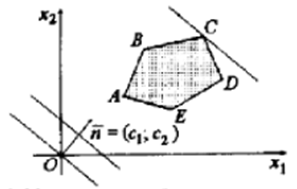
\includegraphics[]{1-2.png}\\
  Рис. 1.1. Многоугольник области допустимых решений\\
\end{center}

Линейная функция при фиксированных значениях $Z(x)=0$ является уравнением прямой линии $c_1x_1+c_2x_2=const$. Прямая, соответствующая данной функции, проходит через начало координат. Другим значениям соответствует прямые параллельные друг другу.

Прямая, уравнение которой получается из целевой функции, если ее приравнять постоянной величине, называется линией уровня.

Вектор нормали уровня $\vec{n}$ имеет координаты c1 и c2.

Если перемещать линию уровня параллельно своему начальному положению в направлении вектора $\vec{n}$, то последней точкой, в которой линия уровня коснется области допустимых решений (ОДР) будет точка с.

Линия уровня, имеющая общие точки с ОДР и расположенная так, что ОДР целиком находится в одной из полуплоскостей называется опорной прямой.

Алгоритм решения задачи линейного программирования:
\begin{enumerate}
	\item Строится область допустимых решений.
	\item Строится вектор $\vec{n}= (c_1, c_2)$ с точкой приложения в начале координат.
	\item Перпендикулярно вектору $\vec{n}$ проводится одна из линий уровня
	\item Линия уровня перемещается параллельно самой себе до положения опорной прямой. На этой прямой находится максимум или минимум функции
\end{enumerate}

\section{Решение индивидуального задания}
Дана задача:\\

\begin{math}
  Z(X)=2x_1+4x_2 \rightarrow  \text{min} \\
  \begin{cases}
    2x_1-x_2 \geq 0\\
    -x_1-x_2 \leq 0\\
    3x_1+7x_2 \leq 40\\
    8x_1-4x_2 \leq 26\\
  \end{cases}\\
  x_1\geq 0, \quad x_2\geq 0
\end{math}\\

Изобразим на плоскости систему координат $Ox_1x_2$ и построим граничные прямые ОДР:\\

\begin{math}
  x_1\geq 0, \quad x_2\geq 0\\
  \begin{cases}
    2x_1-x_2 \geq 0,(1)\\
    -x_1-x_2 \leq 0,(2)\\
    3x_1+7x_2 \leq 40,(3)\\
    8x_1-4x_2 \leq 26,(4)\\
  \end{cases}\\
\end{math}\\

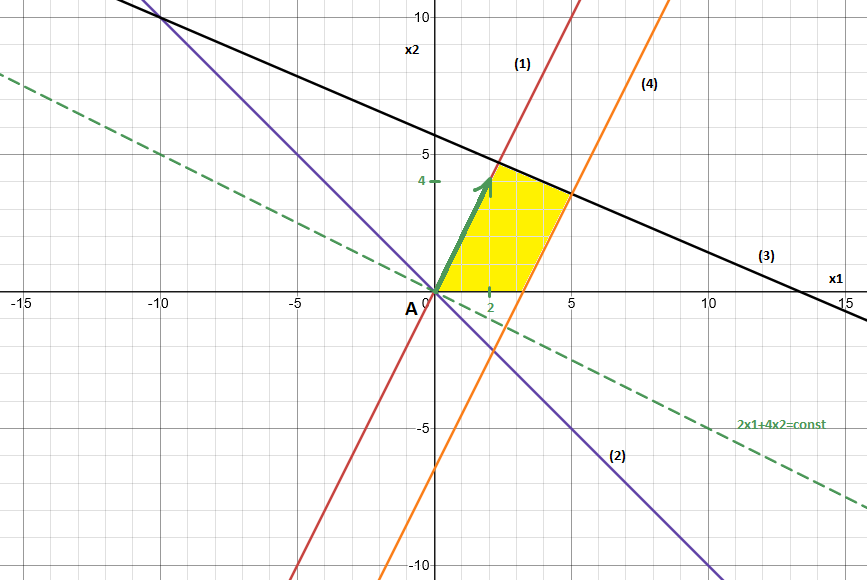
\includegraphics[width=\textwidth]{1-1.png}
\begin{center}
  Рис. 1.2 Область допустимых решений
\end{center}

Для линий уровня $2x_1+4x_2 = \text{const}$ строим нормальный вектор $\vec{n} = (2,4)$ перпендикулярно вектору нормаль построим одну из линий уровня Перемещаем её в направлении вектора $\vec{n}$ до опорной прямой. Для определения координат точки A решаем систему уравнений:\\

\begin{math}
  \begin{cases}
    2x_1-x_2 \geq 0,(1)\\
    -x_1-x_2 \leq 0,(2)\\
  \end{cases}
\end{math}\\

Получаем $x_1 = 0, x_2 = 0$ это и есть оптимальное решение. Минимальное значение целевой функции $Z(X) = 2 \cdot 0 + 4 \cdot 0 = 0$.

\end{document}